\documentclass{article}
\usepackage{graphicx} % Cargamos el paquete graphicx para manejar imágenes
\title{Motores de renderizado en Blender}
\begin{document}
\maketitle

\section{Formatting}
\textit{This text is italicized.}
\textbf{This text is bold.}

\subsection{Equations}
Here is a simple equation:
\[E=mc^2\]

\section{Cycles}
\subsection{Descripción General}
La documentación de Blender define Cycles como el motor basado en físicas para producción. 
Está diseñado para producir resultados basados en la física de forma predeterminada, 
con control artístico y nodos de sombreado flexibles para satisfacer las necesidades 
de producción.

Esto quiere decir que Cycles basa su renderizado en física. Al estar basado en la
física real, los resultados que podemos obtener serán más realistas, pero vamos analizemos
en mayor profundidad su funcionamiento.

\subsection{Componentes de Cycles}
\begin{figure}[h] % "h" significa que LaTeX intentará colocar la imagen aquí
  \centering % Centra la imagen horizontalmente
  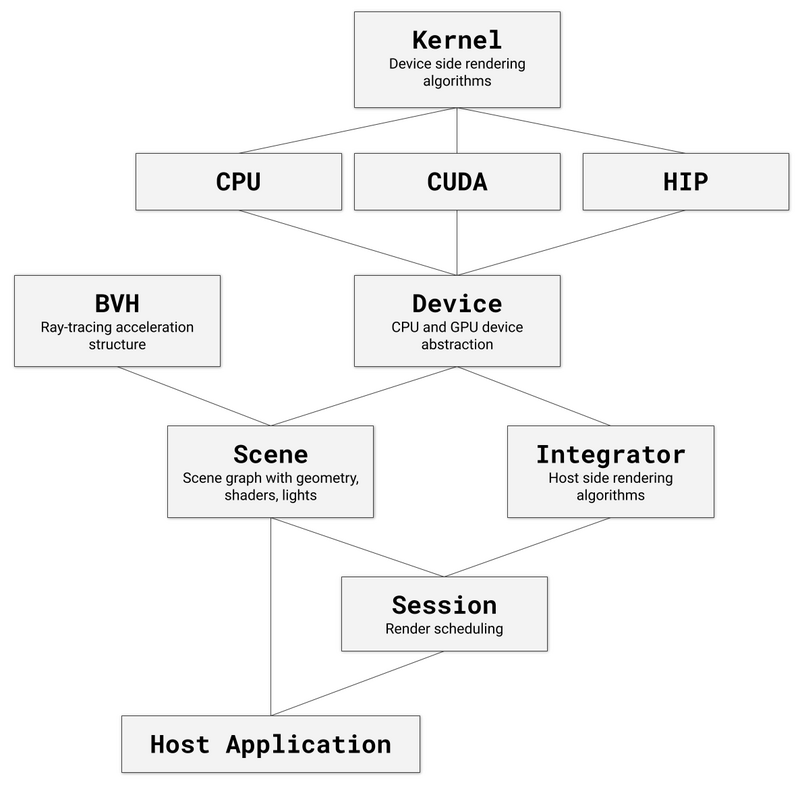
\includegraphics[scale=0.4]{Imagenes/Cycles-modules-architecture.png} % Reemplaza "nombre_de_tu_imagen.png" por el nombre de tu archivo de imagen
  \caption{Descripción general de alto nivel de los módulos de Cycles} % Agrega una descripción
  \label{fig:Cycles_diagram} % Etiqueta para referencias cruzadas
\end{figure}

El diagrama de la figura 1 consiste en una explicación simplificada pero amplia de los componentes 
fundamentales que constituyen el motor de renderizado Cycles. Estos módulos de Cycles son los 
componentes o bloques clave para el motor, las distintas partes del proceso de renderizado que 
realizan funciones específicas. A continuación se procede a explicar cada sección del esquema.

\subsubsection{Kernel: Algoritmos de Renderizado}
Esto representa los algoritmos centrales de renderizado utilizados por Cycles. 
Estos algoritmos son los responsables de los cálculos de renderizado reales que ocurren en el
dispositivo (CPU, GPU u otras unidades de procesamiento). Es decir, son las instrucciones de 
renderizado a nivel más bajo que interactúan directamente con el hardware.

\subsubsection{Opciones de Dispositivos}
Los siguientes tres módulos del esquema representan las diferentes opciones o recursos de un ordenador
que Cycles puede utilizar para realizar su renderizado. Los usuarios elegirán entre ellos según 
sus necesidades y el hardware disponible. La capacidad de utilizar CPUs o GPUs brinda 
flexibilidad en el uso del motor.
\begin{itemize}
  \item CPU: Es una de las opciones de dispositivo disponibles para el renderizado. Cycles puede
  utilizar la CPU (Unidad Central de Procesamiento) para cálculos de renderizado. A menudo es 
  la elección predeterminada cuando no se dispone de una GPU dedicada.
  \item CUDA: es una plataforma de cómputo paralelo y una API desarrollada por NVIDIA. Cycles 
  puede aprovechar las GPU (Unidades de Procesamiento Gráfico) habilitadas para CUDA para el 
  renderizado.
  \item HIP: HIP significa Interfaz de Cómputo Heterogéneo para Portabilidad, y es una API 
  en tiempo de ejecución desarrollada por AMD. Cycles también puede utilizar las GPU de AMD 
  que admiten la API HIP para el renderizado.
\end{itemize}

\subsubsection{Dispositivo: Abstracción de CPU y GPU}
Representa una capa de abstracción que permite a Cycles interactuar tanto con CPUs como 
con GPUs. Proporciona una manera de gestionar y coordinar tareas de renderizado entre estos 
diferentes dispositivos. Permite que Cycles interactúe con la CPU y la GPU sin tener que 
preocuparse por los detalles específicos de la estructura de cada uno.

\subsubsection{BVH: Estructura de aceleración para trazado de rayos}
BVH significa Jerarquía de Volumen Delimitador, que es una estructura de aceleración utilizada 
en el trazado de rayos. Cycles utiliza BVH como un componente crítico para acelerar los cálculos
de trazado de rayos, optimizando el rendimiento de renderizado.

\subsubsection{Escena: Grafo de escena con geometría, shaders, luces}
Esto representa la gestión de la escena por parte de Cycles. Incluye información sobre la 
escena 3D, como la geometría (objetos), shaders (materiales) y configuraciones de iluminación.

\subsubsection{Integrador: Algoritmos de renderizado en el lado del anfitrión}
Además de los mencionados algoritmos de renderizado en el lado del dispositivo, se tratan ahora
los algoritmos de renderizado en el lado del anfitrión (host). Consiste de las instrucciones
propias del motor de renderizado, que se ejecutan directamente en el host (la CPU).

\subsubsection{Sesión: Programación de renderizado}
Consiste en la gestión de sesión y la programación de componentes de Cycles. Coordina el 
proceso de renderizado y gestiona cómo se programan y ejecutan las tareas de renderizado.

\subsubsection{Aplicación host}
Suele ser el programa de Blender en sí. Es la interfaz de usuario y el entorno donde el 
diseñador interactúa con Cycles para crear y renderizar escenas 3D.


\subsection{Uso de Cycles}
Una vez analizado el funcionamiento de este motor, veamos más información acerca de su uso para
diseñadores y desarrolladores que interactuan directamente con Blender.

(A partir de aquí, el texto es una traducción del libro que tenemos como referencia).

\subsubsection{Ray Tracing}
El motor de renderizado Cycles utiliza ray-tracing para intentar imitar el comportamiento 
real de una superficie lo más fielmente posible.

En Cycles, todos los materiales que describen propiedades de superficie tienen una Función 
de Distribución de Dispersión Bidireccional (BSDF), que es una función matemática general 
que describe la forma en que la luz se dispersa en una superficie en el mundo real. También es
la fórmula que utilizan trazadores de rayos como lo es Cycles, para calcular la representación 
de un objeto en un entorno virtual. Básicamente, los rayos de luz se disparan desde la cámara. 
Rebotan en los objetos de la escena y siguen rebotando hasta llegar a una fuente de luz o a un 
fondo vacío (que, en Cycles, también puede emitir luz). Por esta razón, un trazador de rayos 
puro como Cycles puede representar en tiempos razonables un objeto en un entorno abierto. 
Los tiempos de representación aumentan considerablemente para espacios cerrados, por ejemplo, 
muebles dentro de una habitación, porque los rayos de luz pueden rebotar en el suelo, el techo 
y las paredes muchas veces antes de llegar a una o varias fuentes de luz.

Es necesario tener en cuenta que la velocidad de renderización en Cycles depende del dispositivo
que se utilice para representar las escenas, como se explicaba anteriormente. Esto significa que
se permite al usuario decidir utilizar la potencia de su CPU o la potencia de su tarjeta gráfica. 

\subsection{Conclusiones sobre Cycles}
Es un motor de renderizado que usa ray-tracing.
Para calcular cómo “rebota” la luz en la superficie de un objeto, se usa su propiedad BDSF.
Puede usar CPU o GPU.

\section{Eevee}
Eevee se introdujo en la versión 2.8 de Blender. 

\textit{“EEVEE is a GPU rasterize based renderer. It uses gaming rasterizer techniques to 
render very fast, but uses higher quality renderings as we don't need to stick to a minimum 
framerate.”}

Esta citación quiere decir que el motor de renderizado Eevee se basa en rasterización.
La rasterización es un proceso fundamental en IG que se utiliza para convertir objetos 
tridimensionales en una representación bidimensional. Para mostrar estos objetos en una
pantalla (2D), es necesario proyectarlos en el plano. La proyección es el proceso de 
determinar cómo se ven los objetos 3D desde la perspectiva de una cámara virtual.

El proceso de rasterización hace una estimación de la manera en que la luz interactua con los
objetos y materiales haciendo uso de diversos algoritmos. Al ser una estimación, será siempre
menos realista que un resultado conseguido por otros métodos como ray-tracing.

¿Cómo hace entonces Eevee para mostrar los elementos de la escena? La respuesta es el uso de
shaders. Eevee depende de los shaders para simular la apariencia de materiales y la iluminación.
Los shaders son programas que describen cómo la superficie de un objeto interactúa con la luz. 
En Blender, estos son los BDSFs (Funciones de Difusión de Superficie Bidireccional). 
Eevee admite una amplia variedad de tipos de shaders, incluidos los shaders PBR (Renderizado 
Basado en Física) para materiales realistas.

\subsection{Uso de Eevee}
Es un motor que está diseñado para producir renders en tiempo real y es especialmente adecuado
para tareas que requieren interactividad y velocidad en la vista previa de escenas 3D. 
Para lograr esto, Eevee utiliza técnicas de rasterización y sombreado en tiempo real 
para generar imágenes rápidamente. Esto incluye el cálculo de sombras en tiempo real, que son 
una representación simplificada de cómo la luz interactúa con los objetos en la escena.

Se crean los materiales de la misma manera que para Cycles, pero estos se pueden previsualizar 
en tiempo real.

\subsection{Conclusiones sobre Eevee}
Este motor de renderizado utiliza el método de la rasterización. En blender, utilizamos
materiales con propiedades BDSF para indicar cómo se refleja la luz.

\section{Diferencias entre Eevee y Cycles}
La principal diferencia entre estos dos motores de renderizado se reduce a uso de ray tracing 
contra uso de rasterización.
En Cycles, vemos el resultado real directamente, pues se replica el comportamiento de la luz, 
ofreciendo una visión igual o muy similar a la que tendría el ojo humano en un entorno físico.
Cuando se define un material BDSF en Blender para su renderizado con Cycles, se determinan las
propiedades del material, y el motor se encargará de simular el comportamiento de la luz al 
incidir en él. 
En Eevee debemos hacer algunas “trampas” para simular los mismos efectos en un material. Se 
debe indicar de manera artificial con shaders cómo va a reflejar la luz en esa superficie, 
en lugar de indicar únicamente las propiedades de dicho material.

\end{document}
